% =====================================================================
%  Diagonality: The Best of Both Worlds
%  AWS World Sports Innovation Cup 2026 - Challenge 2: 3D Football Data
%
%  Compile on Overleaf (pdfLaTeX). Bibliography: BibTeX (references.bib).
%  Final PDF -> docs/Challenge_3D_Football_Data.pdf
% =====================================================================
\documentclass[11pt]{article}

\usepackage[utf8]{inputenc}
\usepackage[T1]{fontenc}
\usepackage{lmodern}
\usepackage[a4paper,margin=2.4cm]{geometry}
\usepackage{graphicx}
\usepackage{amsmath,amssymb}
\usepackage{booktabs}
\usepackage{xcolor}
\usepackage{caption}
\usepackage{subcaption}
\usepackage{microtype}
\usepackage[numbers,sort&compress]{natbib}
\usepackage[colorlinks=true,linkcolor=black,citecolor=black,urlcolor=blue]{hyperref}

\graphicspath{{figures/}}
\captionsetup{font=small,labelfont=bf}

% --- video reference helper: links a figure to its repo video --------
\newcommand{\repobase}{https://github.com/jaime-oriol/Diagonality\_3D/blob/main}
\newcommand{\videoref}[2]{\textcolor{blue}{\href{\repobase/#1}{\texttt{#2}}}}

\title{\textbf{Diagonality: The Best of Both Worlds}\\[4pt]
\large Quantifying Football's Progression--Safety Trade-off with 3D Skeleton
Tracking and Orientation-Aware Pitch Control}

\author{Jaime Oriol\\
\small AWS World Sports Innovation Cup 2026 --- Challenge 2: Unlock the Power of 3D Football Data}
\date{}

\begin{document}
\maketitle

% =====================================================================
\begin{abstract}
\noindent
Diagonality --- favouring oblique passes, carries and runs over straight
vertical or horizontal ones --- is among the most discussed yet least
quantified concepts in modern football tactics. Spielverlagerung frames it
as \emph{``the best of both worlds''}: a diagonal action is claimed to
combine the progression of a vertical pass with the safety of a horizontal
one. Testing this claim was impossible while tracking data captured
positions but not body orientation, which had to be proxied from the
velocity vector ($30$--$50^\circ$ error). We use TRACAB 3D skeleton data
from five Bundesliga 2025--26 matches (21 keypoints per player at
50\,Hz) --- the first dataset with directly measured head, shoulder and hip
orientation --- to build a four-stage orientation-aware framework: a
per-defender probabilistic vision model adapted from Bekkers; an
Orientation-Aware Pitch Control Function built from anisotropic reach
fields; the \emph{Diagonal Opportunity Surface} (DOS), a pitch map of where
a diagonal delivery buys the most control; and a cognitive scanning gate.
Across 6{,}923 passes, carries and take-ons, diagonal actions are
Pareto-optimal on the progression--safety plane: they retain possession far
more often than vertical actions (63\% vs 44\%) while gaining almost as
much expected threat, and produce a positive xT outcome 82\% of the time
(vs 74\% forward, 32\% sideways). DOS predicts xT gain after controlling
for distance, pressure and defender counts (Mann--Whitney $p<10^{-25}$;
logistic regression $p<10^{-4}$). Mechanistically, diagonal actions disrupt
the defensive block on both structural axes combined and hand the receiver
a body already oriented to progress, with more passing options in view. We
release DOS as a coach-facing, per-opponent map.
\end{abstract}

% =====================================================================
\section{Introduction}
\label{sec:intro}

For two decades coaching discourse has been dominated by a single
imperative: \emph{play forward}. Progress the ball toward goal whenever
possible; mitigate the risk with counter-pressing. Its mirror image is
\emph{keep the ball} --- recycle horizontally, accept no progression in
exchange for near-certain retention. These are not two philosophies but the
two poles of one axis: \textbf{progression versus safety}. A vertical pass
maximises progression and risk; a horizontal pass maximises safety and
sterility. Spielverlagerung's 2025 deep-dive on
\emph{Diagonality}~\citep{spielverlagerung2025} argues that there exists an
optimum \emph{between} the poles --- the diagonal --- which captures
``the progression of a vertical pass and the safety of a horizontal one:
progress with less risk, control with the chance to react.'' Jamie
Hamilton's \emph{Diagonalist Manifesto}~\citep{hamilton2024} reframes the
same idea as a vectorial logic in which the diagonal reception is the point
of maximum tactical multiplicity.

Diagonality has never been quantified because it is fundamentally about
\emph{body orientation}, and tracking data captured only positions.
Orientation had to be proxied from the velocity vector, introducing
$30$--$50^\circ$ of error~\citep{arbues2020} that drowns the signal.
\citet{bekkers2026} reduced this to $\sim$27$^\circ$ using broadcast pose
estimation. We instead use TRACAB optical 3D skeleton tracking: real head,
shoulder and hip keypoints at 50\,Hz. This is the first dataset that makes
the diagonality hypothesis computationally testable.

%% PLAN intro: cierre con (i) research question, (ii) las 4 contribuciones,
%% (iii) un parrafo "roadmap" del paper.
\paragraph{Contributions.}
%% PLAN: lista de 4 - (1) framework orientation-aware sobre skeleton 3D real;
%% (2) DOS, surface nueva, validada; (3) la evidencia del trade-off; (4)
%% deliverable coach-facing. Redactar como parrafo o itemize.

% =====================================================================
\section{Related Work}
\label{sec:related}

%% PLAN: 1-2 parrafos. Pitch control (Taki2000, Spearman2017/2018,
%% Fernandez2018, fernandez2020soccermap) -> vision (Bekkers2026) -> defensive
%% disruption (Goes2019, Forcher2021/2024) -> action value (Singh2018,
%% Decroos2019, Anzer2022) -> tactical theory (Spielverlagerung, Hamilton) ->
%% biomechanics (Vater2024, DosSantos2018). Cerrar: nadie ha cruzado vision +
%% pitch control + disrupcion + diagonalidad. Esa interseccion es el aporte.

% =====================================================================
\section{Data}
\label{sec:data}

We analyse five Bundesliga 2025--26 matches provided by DFL / Sportec
Solutions with TRACAB GEN5/GEN6 3D skeleton tracking: Bayern 5--0 Hamburg,
Dortmund 3--3 Stuttgart, Frankfurt 0--3 Bayern, Frankfurt 3--4 Union, and
Union 2--2 Bayern ($\sim$20.6\,GB total). Each frame provides, at 50\,Hz,
\textbf{21 three-dimensional keypoints per player} (ears, nose, shoulders,
neck, elbows, wrists, hips, pelvis, knees, ankles, heels, toes) in metres
from the pitch centre. From the keypoints we derive the real orientation of
each player on three independent signals: head yaw (perpendicular to the
ear--ear axis), shoulder facing (perpendicular to the shoulder axis) and hip
facing (perpendicular to the hip axis). Player position is the pelvis
keypoint.

Skeleton data is paired with DFL enriched event data (\texttt{kpi\_data}):
$\sim$1{,}190 passes and $\sim$338 carries per match, each carrying
\texttt{PlayAngle}, expected pass probability (xP), pressure, defender
counts and a \texttt{SyncedFrameId} that aligns the event to the skeleton.
Successful take-ons are recovered from the \texttt{TacklingGame} events.
After synchronisation and filtering we evaluate \textbf{6{,}923 on-ball
actions} (5{,}128 passes, 1{,}604 carries, 191 take-ons).

%% PLAN data: anadir (i) frase sobre la ventaja de orientacion medida vs
%% proxy; (ii) clasificacion direccional DFL (forward 0-22 deg, diagonal
%% 23-67, sideways 68-112, backward >112); (iii) opcional: tabla mini de los
%% 5 partidos.

% =====================================================================
\section{Methods}
\label{sec:methods}

The framework runs in four stages. Each player is described by real 3D
orientation; from orientation we build what the player \emph{sees}
(Sec.~\ref{sec:vision}); from orientation-aware biomechanics we build what
the player can physically \emph{reach} (Sec.~\ref{sec:ppcf}); the two
combine into the Diagonal Opportunity Surface (Sec.~\ref{sec:dos}); a
cognitive gate restricts it to what the on-ball player can actually
perceive (Sec.~\ref{sec:gate}).

\subsection{Defender Orientation and the Vision Model}
\label{sec:vision}

%% PLAN: Bekkers FOV 120 deg, decaimiento gaussiano radial+angular modulado
%% por velocidad; oclusion por torso con shoulder_width REAL del skeleton
%% (Bekkers usa ancho fijo). Salida: V_i(x,y) en [0,1] por defensor.
\begin{figure}[t]
  \centering
  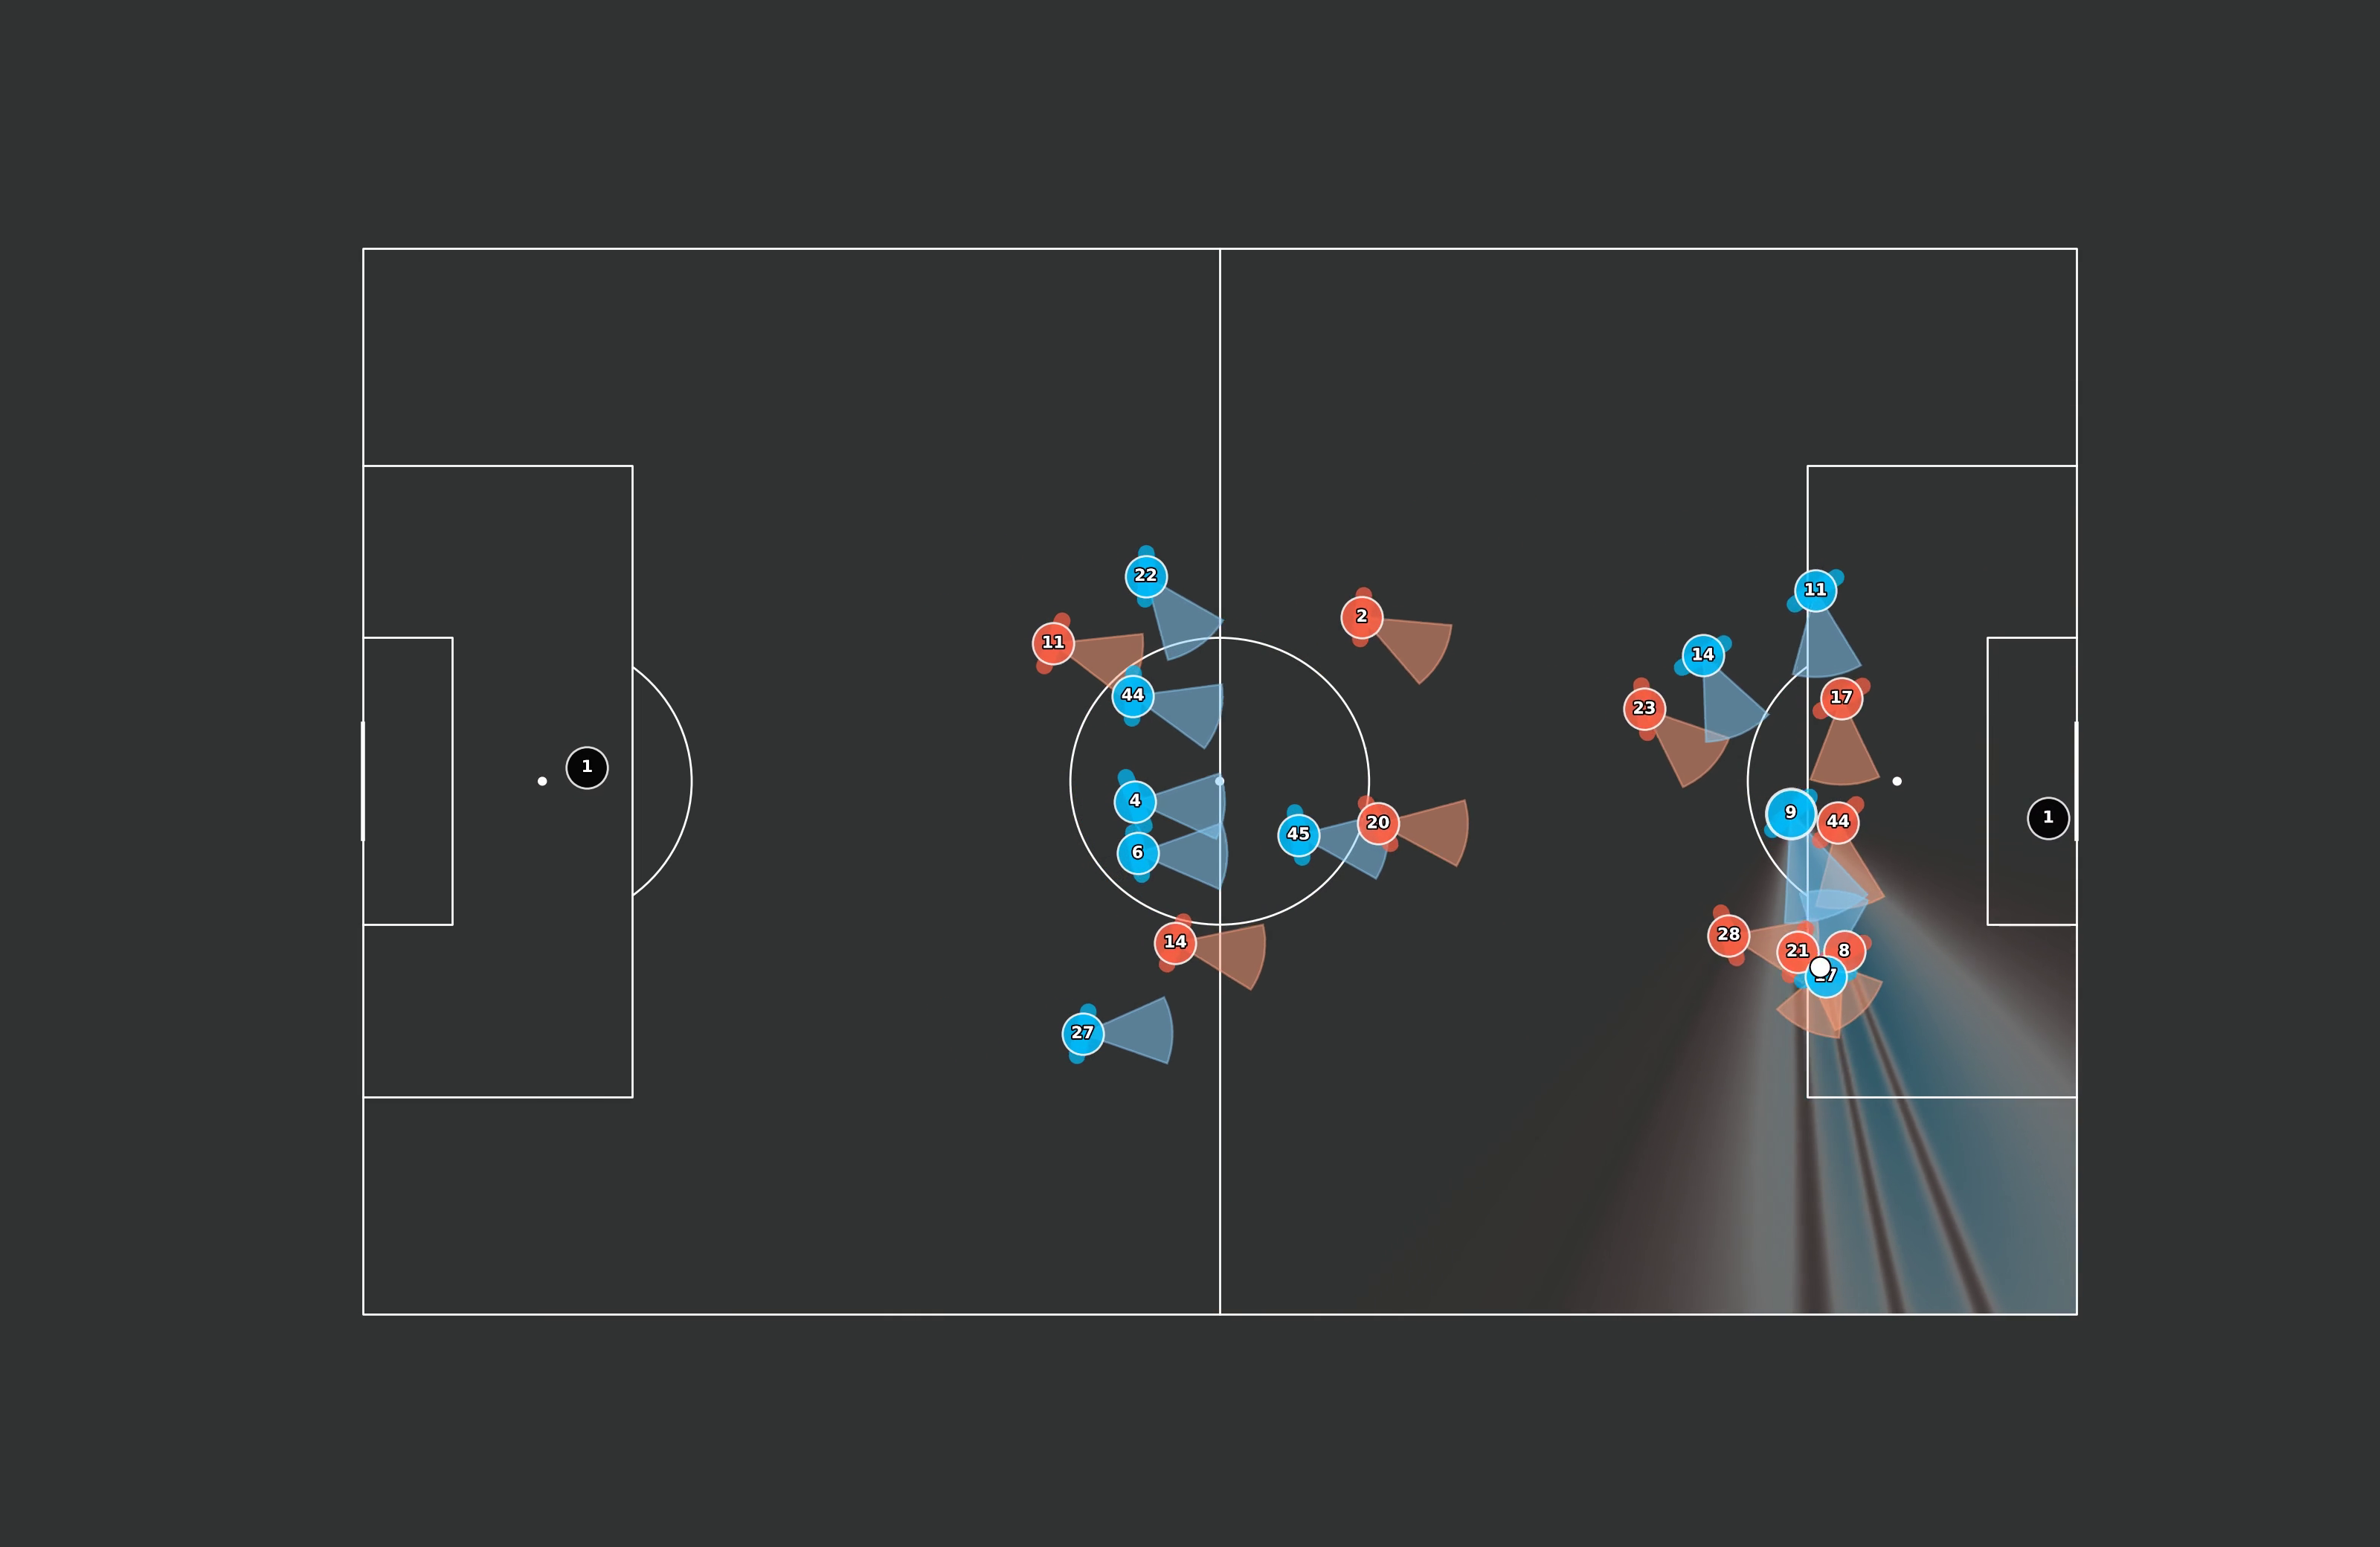
\includegraphics[width=0.92\textwidth]{impl_vision.png}
  \caption{\textbf{Vision model.} Per-player field of view (adapted
  from~\citet{bekkers2026}): a 120$^\circ$ probabilistic cone with
  speed-dependent radial and angular decay, plus torso occlusion computed
  from the \emph{real} shoulder width of each occluder.
  Video: \videoref{aws\_results/videos/kane\_vision.mp4}{kane\_vision.mp4}.}
  \label{fig:vision}
\end{figure}

\subsection{Orientation-Aware Pitch Control}
\label{sec:ppcf}

%% PLAN: cada jugador = gaussiana 2D anisotropa; sigma derivada del delay
%% biomecanico orientado: rt(theta) Vater2024 + cod(theta) DosSantos2018
%% aplicados al shoulder_angle real. El blob del defensor tiene un HUECO en
%% su blind spot. Ecuaciones theta_i -> delay_i -> reach_i -> sigma_i.
%% Agregacion por equipo -> ppcf_att / ppcf_def.
\begin{figure}[t]
  \centering
  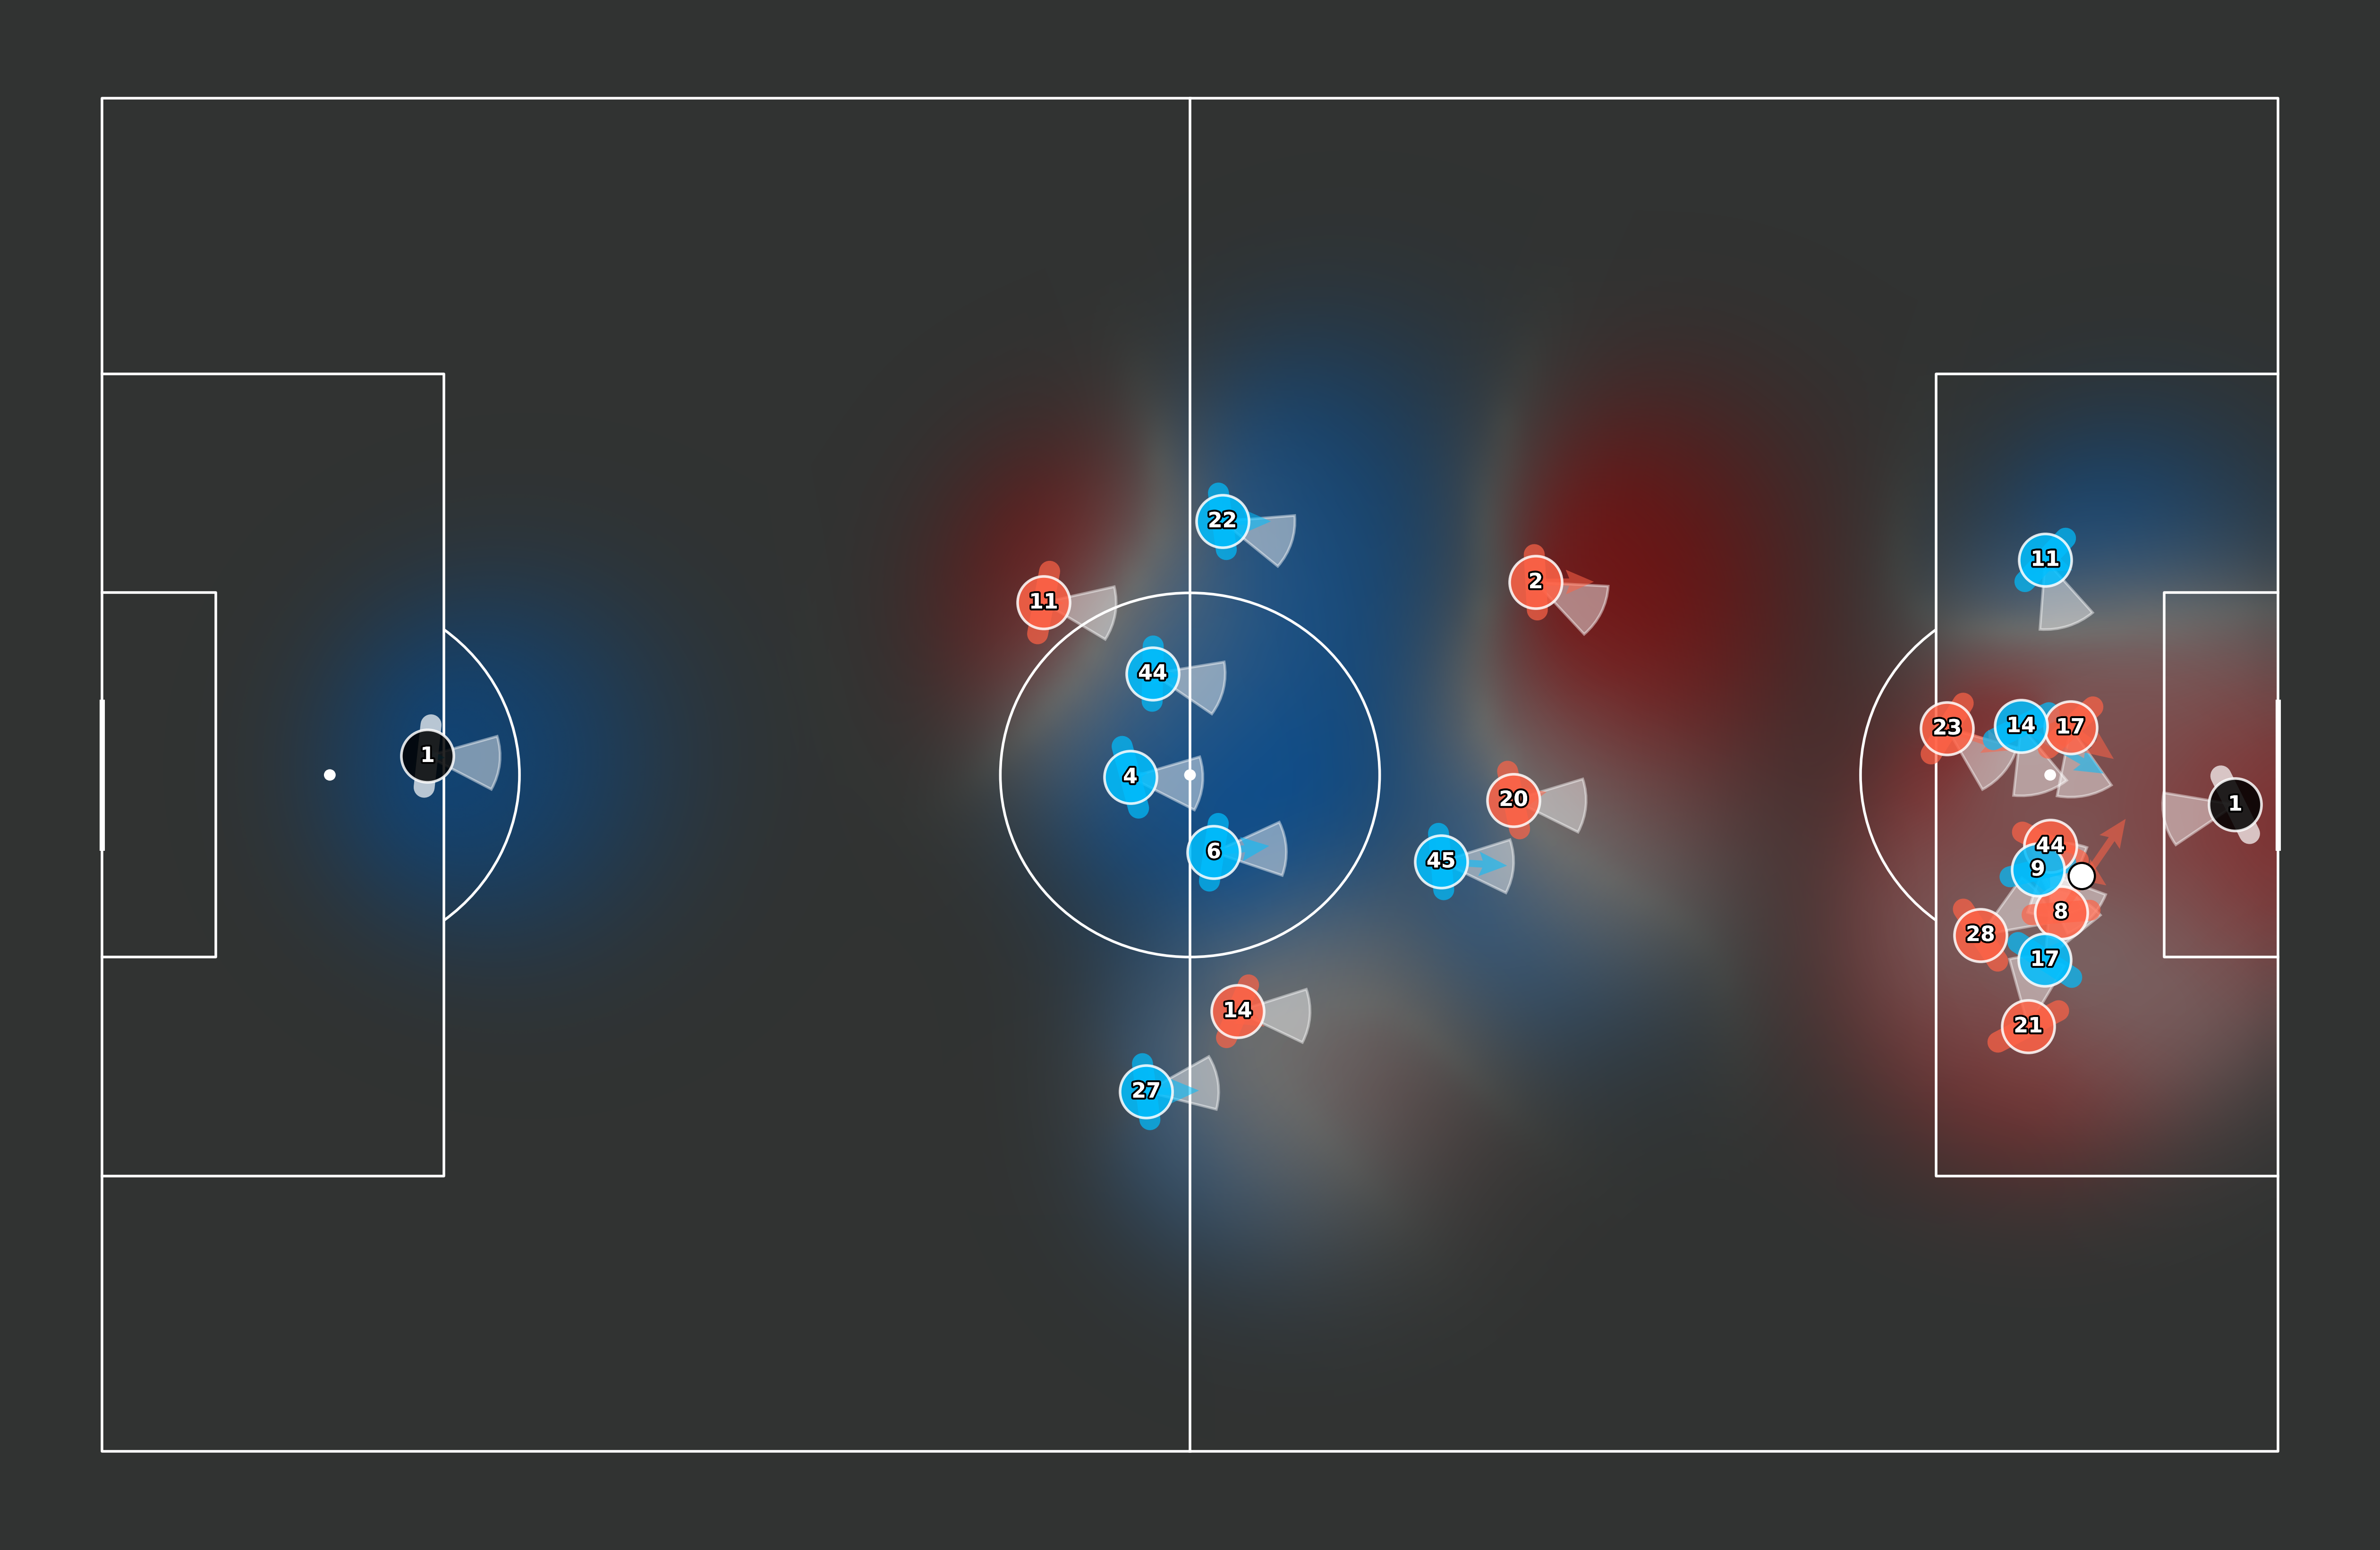
\includegraphics[width=0.92\textwidth]{impl_ppcf.png}
  \caption{\textbf{Orientation-Aware Pitch Control.} Each player is an
  anisotropic reach field whose width follows the orientation-aware
  reaction delay (Vater RT + Dos'Santos change-of-direction deficit applied
  to the real shoulder angle). A defender with the threat in his blind spot
  has a visible hole in his control field.
  Video: \videoref{aws\_results/videos/kane\_ppcf.mp4}{kane\_ppcf.mp4}.}
  \label{fig:ppcf}
\end{figure}

\subsection{The Diagonal Opportunity Surface (DOS)}
\label{sec:dos}

%% PLAN: DOS(x,y) = max(ppcf_att diagonales) - max(ppcf_att forwards).
%% Mecanismo: defensores que NO ven la amenaza sufren detection delay extra
%% (awareness = 0.7 V_attacker + 0.3 V_passer, modulado por velocidad y
%% angulo). DOS = mapa de donde la entrega diagonal compra mas control.
\begin{figure}[t]
  \centering
  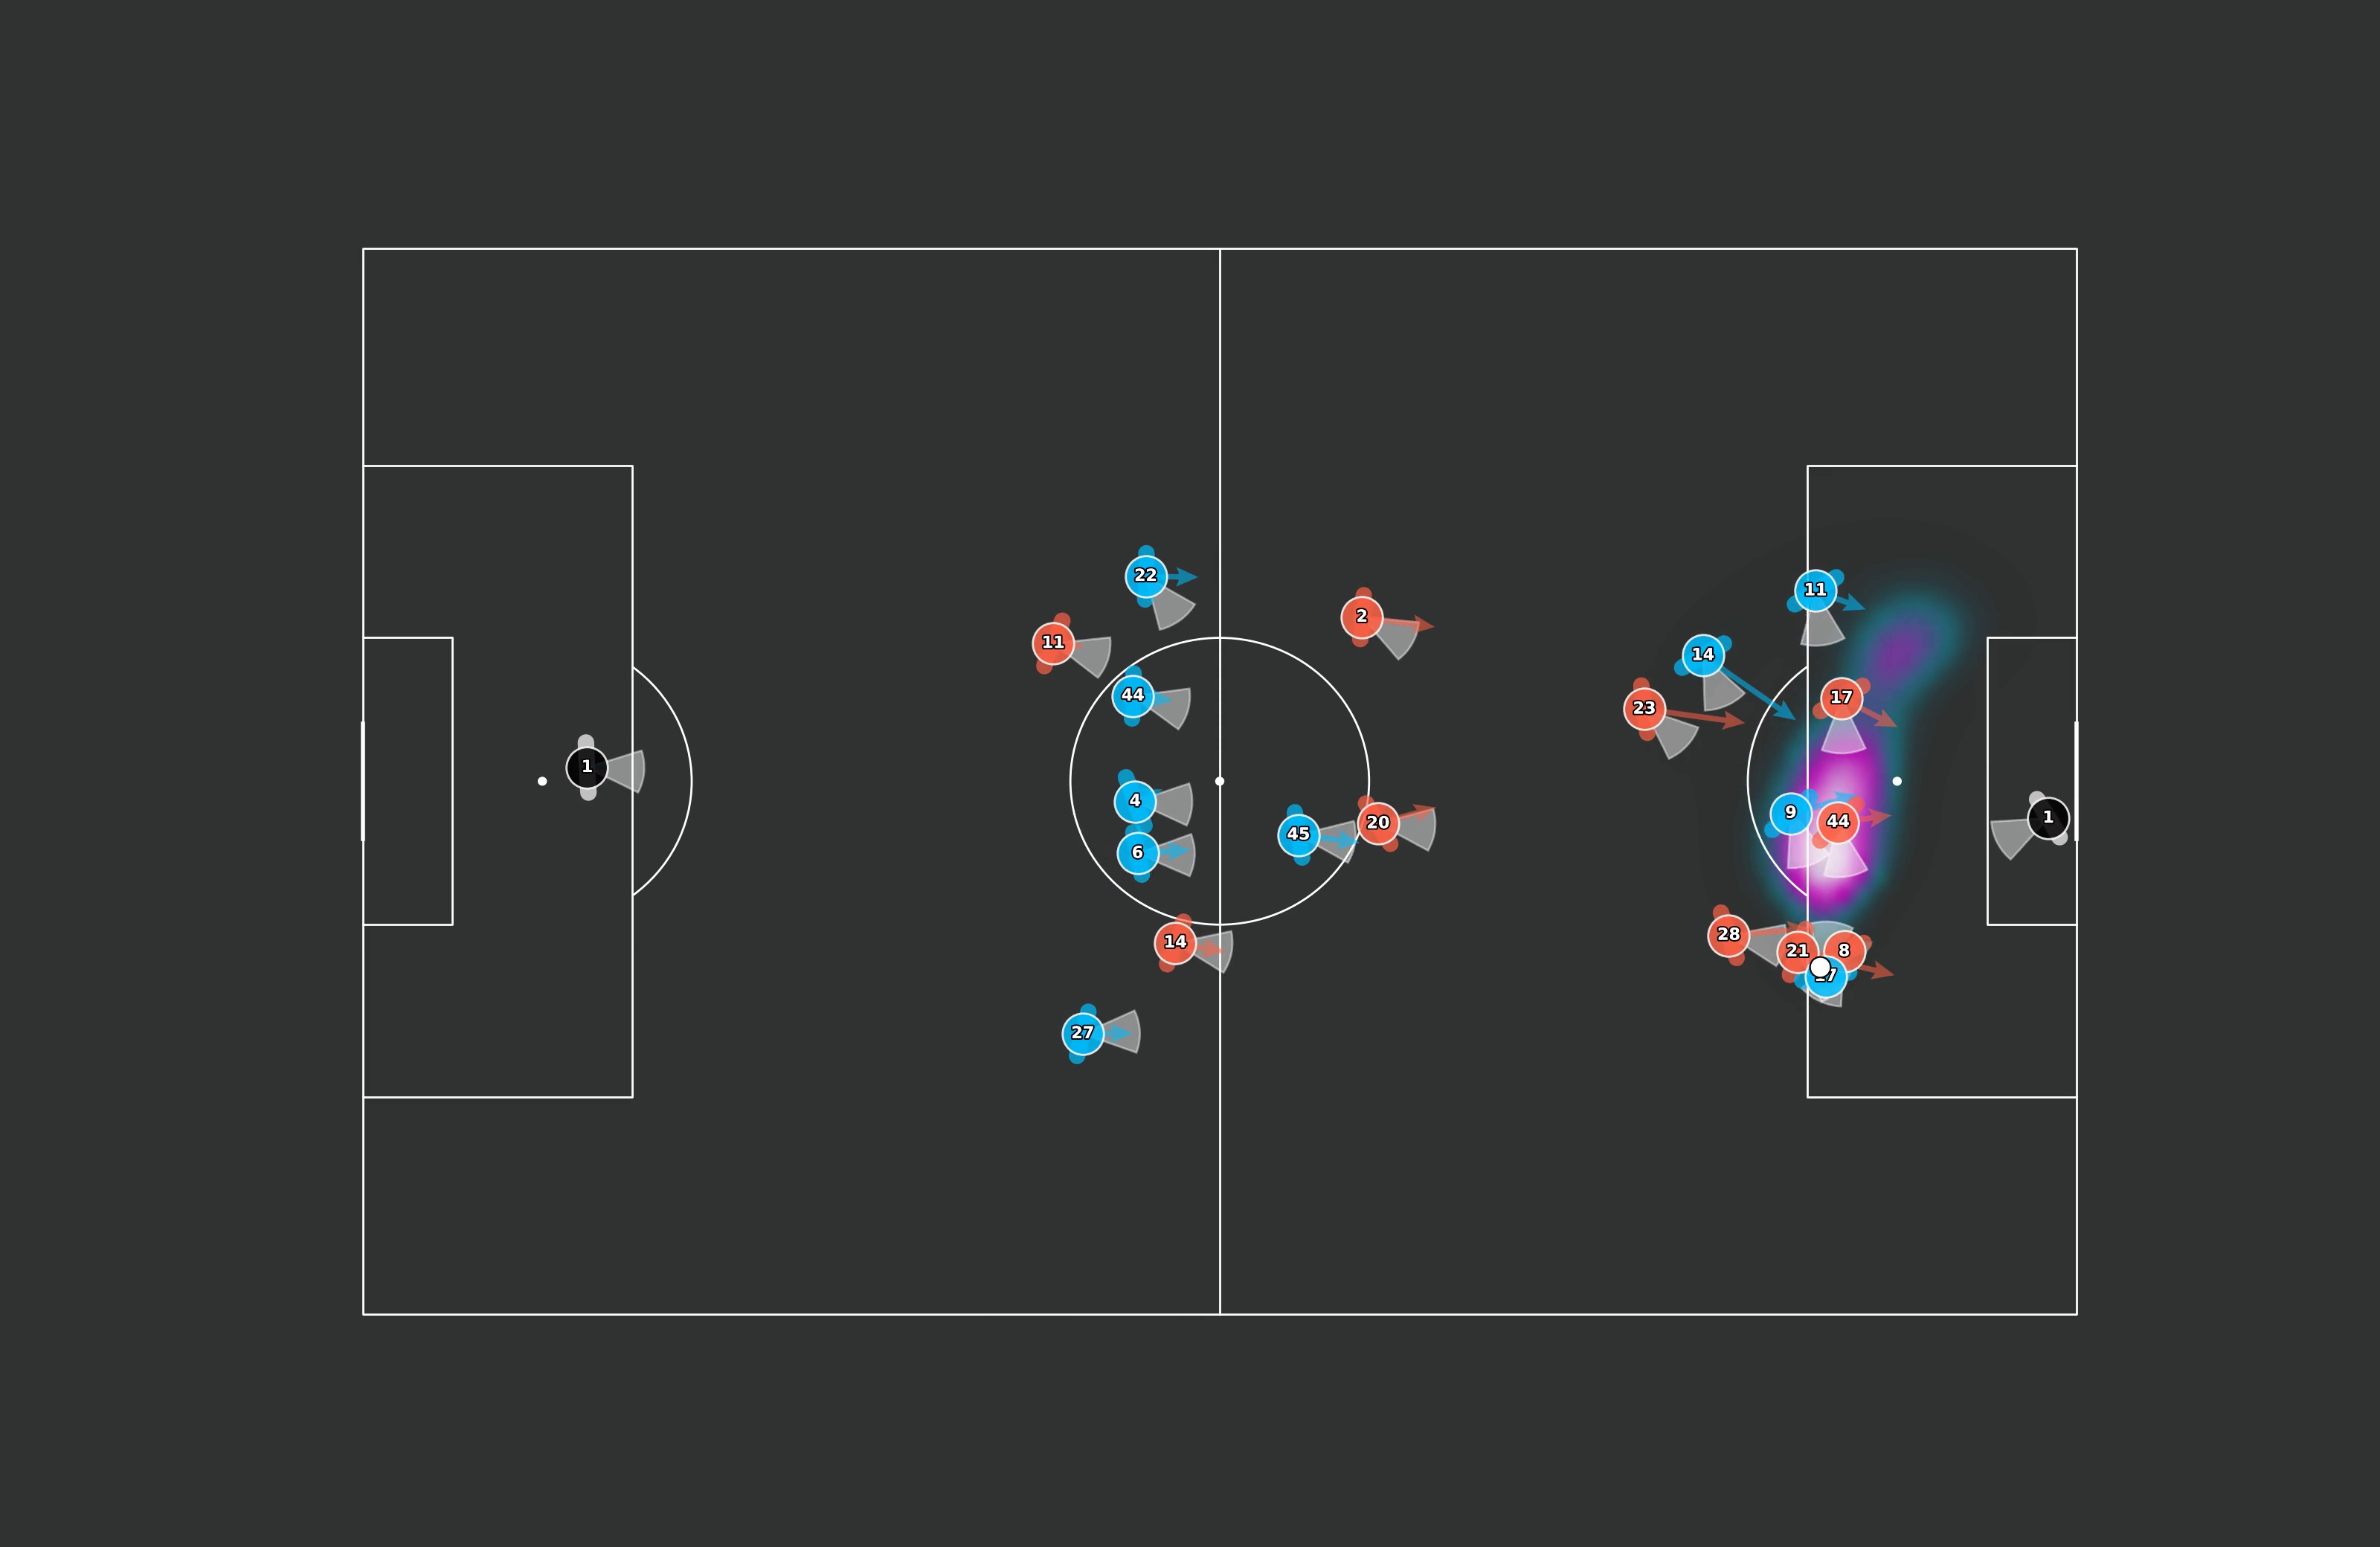
\includegraphics[width=0.92\textwidth]{impl_dos.png}
  \caption{\textbf{Diagonal Opportunity Surface.} For every cell, DOS is the
  extra attacker pitch control bought by the best diagonal delivery over the
  best orthogonal one, given the defenders' real orientation.
  Video: \videoref{aws\_results/videos/kane\_dos.mp4}{kane\_dos.mp4}.}
  \label{fig:dos}
\end{figure}

\subsection{The Cognitive Scanning Gate}
\label{sec:gate}

%% PLAN: possession timeline frame-exacta -> on-ball owner por frame ->
%% scanning memory (FOV Bekkers + 2.5s de memoria con decaimiento). DOS solo
%% se pinta donde el portador VE o ha escaneado. Convierte una metrica
%% god-eye en accionable.

\subsection{Event-Level Metrics and Validation Design}
\label{sec:metrics}

%% PLAN: cadena de enrichment - theta (defender + receiver), D-Def (Goes/
%% Forcher + PCA -> PC1 long / PC2 lat), xT-delta (Singh2018) como outcome
%% causal-fair. CRITICO: el modelo DOS no recibe xG/xT/labels -> los outcomes
%% son independientes. Memory-safe (chunked pyarrow). 136 tests.

% =====================================================================
\section{Results}
\label{sec:results}

\subsection{The Progression--Safety Trade-off}
\label{sec:res-tradeoff}

Table~\ref{tab:tradeoff} is the central result. Forward actions sit at the
progression pole: highest expected-threat gain, but the lowest retention
(44\%) --- ``vertical gets you killed or crowned''. Sideways actions sit at
the safety pole: highest retention (78\%) but \emph{negative} mean xT ---
safe yet sterile. \textbf{Diagonal actions are neither pole and beat both as
a compromise}: they retain the ball far more often than vertical actions
while gaining almost as much expected threat, and they produce a positive
xT outcome 82\% of the time --- the highest of the three classes. This is
``the best of both worlds'' made measurable.

\begin{table}[h]
  \centering
  \caption{The progression--safety trade-off across 6{,}923 on-ball
  actions. Diagonal is Pareto-optimal: not the extreme on either pole, but
  the best joint outcome. (xT $\Delta$: mean Karun~Singh expected-threat
  change; retention: ball kept; xT$>$0: share of actions that gain threat.)}
  \label{tab:tradeoff}
  \begin{tabular}{lrrrr}
    \toprule
    Direction & $n$ & xT $\Delta$ (progression) & Retention (safety) & xT$>$0 rate \\
    \midrule
    Forward (vertical)    & 1{,}137 & $+0.0028$           & 44\%            & 74\% \\
    Sideways (horizontal) & 3{,}514 & $-0.0012$           & \textbf{78\%}   & 32\% \\
    \textbf{Diagonal}     & 2{,}272 & $+0.0027$           & 63\%            & \textbf{82\%} \\
    \bottomrule
  \end{tabular}
\end{table}

%% PLAN: anadir la figura "Pareto plane" (scatter progresion vs retencion,
%% un punto por clase) - pendiente de generar (script o TikZ).

\subsection{DOS Predicts Threat Gain}
\label{sec:res-dos}

%% PLAN: DOS validado contra outcomes que el modelo NUNCA vio. MWU DOS mas
%% alto cuando xT>0: p=1.16e-25 (carries rbc=+0.40, p=1.2e-36). Logistica
%% controlada (distancia, presion, n defensores): dos coef +10.86, p=2.6e-5.
%% Quintiles: tasa xT>0 sube monotona 46% -> 63%.
\begin{figure}[t]
  \centering
  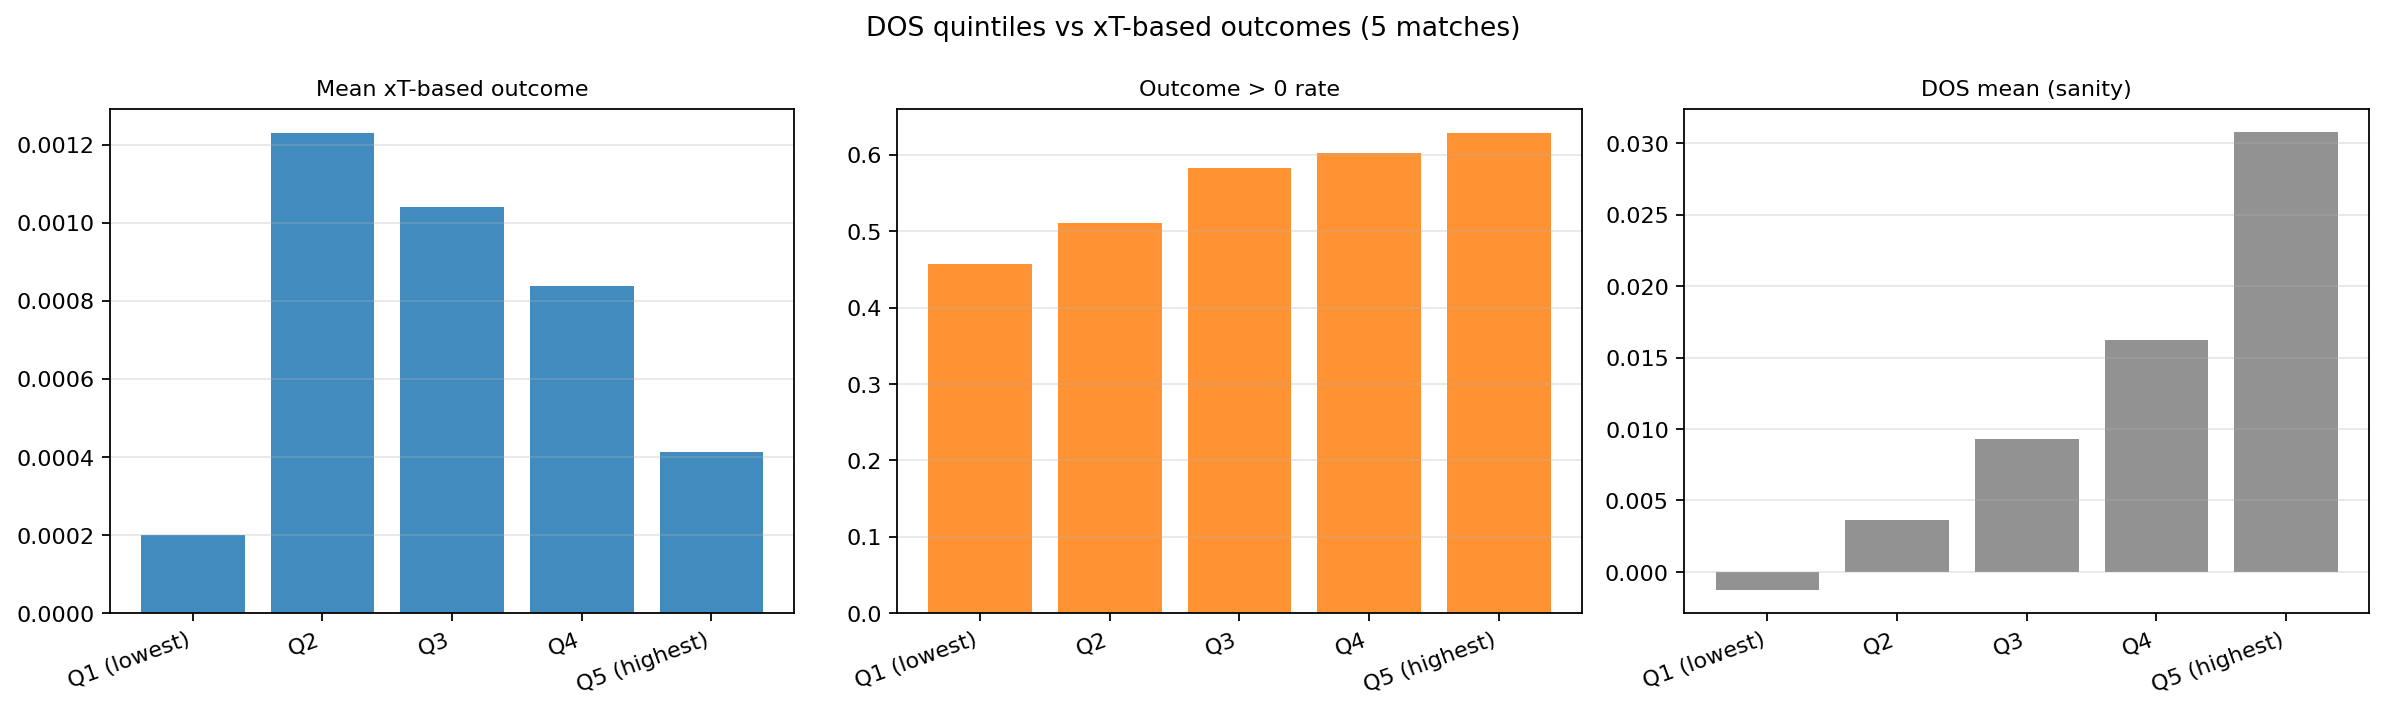
\includegraphics[width=0.97\textwidth]{results_quintiles.png}
  \caption{\textbf{DOS predicts value.} Across DOS quintiles the rate of
  positive expected-threat outcomes rises monotonically (centre). The model
  receives no xG, no xT and no outcome labels --- DOS and xT are
  mathematically independent.}
  \label{fig:quintiles}
\end{figure}

\subsection{Mechanism I --- The Defender}
\label{sec:res-defender}

%% PLAN: por que la diagonal puede hacer trampa al trade-off, lado defensa.
%% D-Def descompuesto: PC1 longitudinal, PC2 lateral. Diagonal NO es el
%% maximo de un eje (forward domina PC1, ~empata) PERO tiene el PC1+PC2
%% COMBINADO mas alto (mediana 2.91 vs 2.62 forward, p=2e-4) y es la
%% especialista lateral (PC2, p=7e-12). Honesto: el balance bi-axial es
%% plano - la diagonal no rompe "los dos por igual", rompe MEJOR los dos
%% juntos. theta: forward desorienta mas (51.7 deg) que diagonal (43.9) -
%% encaja: theta traza el polo riesgo, no contradice.
\begin{figure}[t]
  \centering
  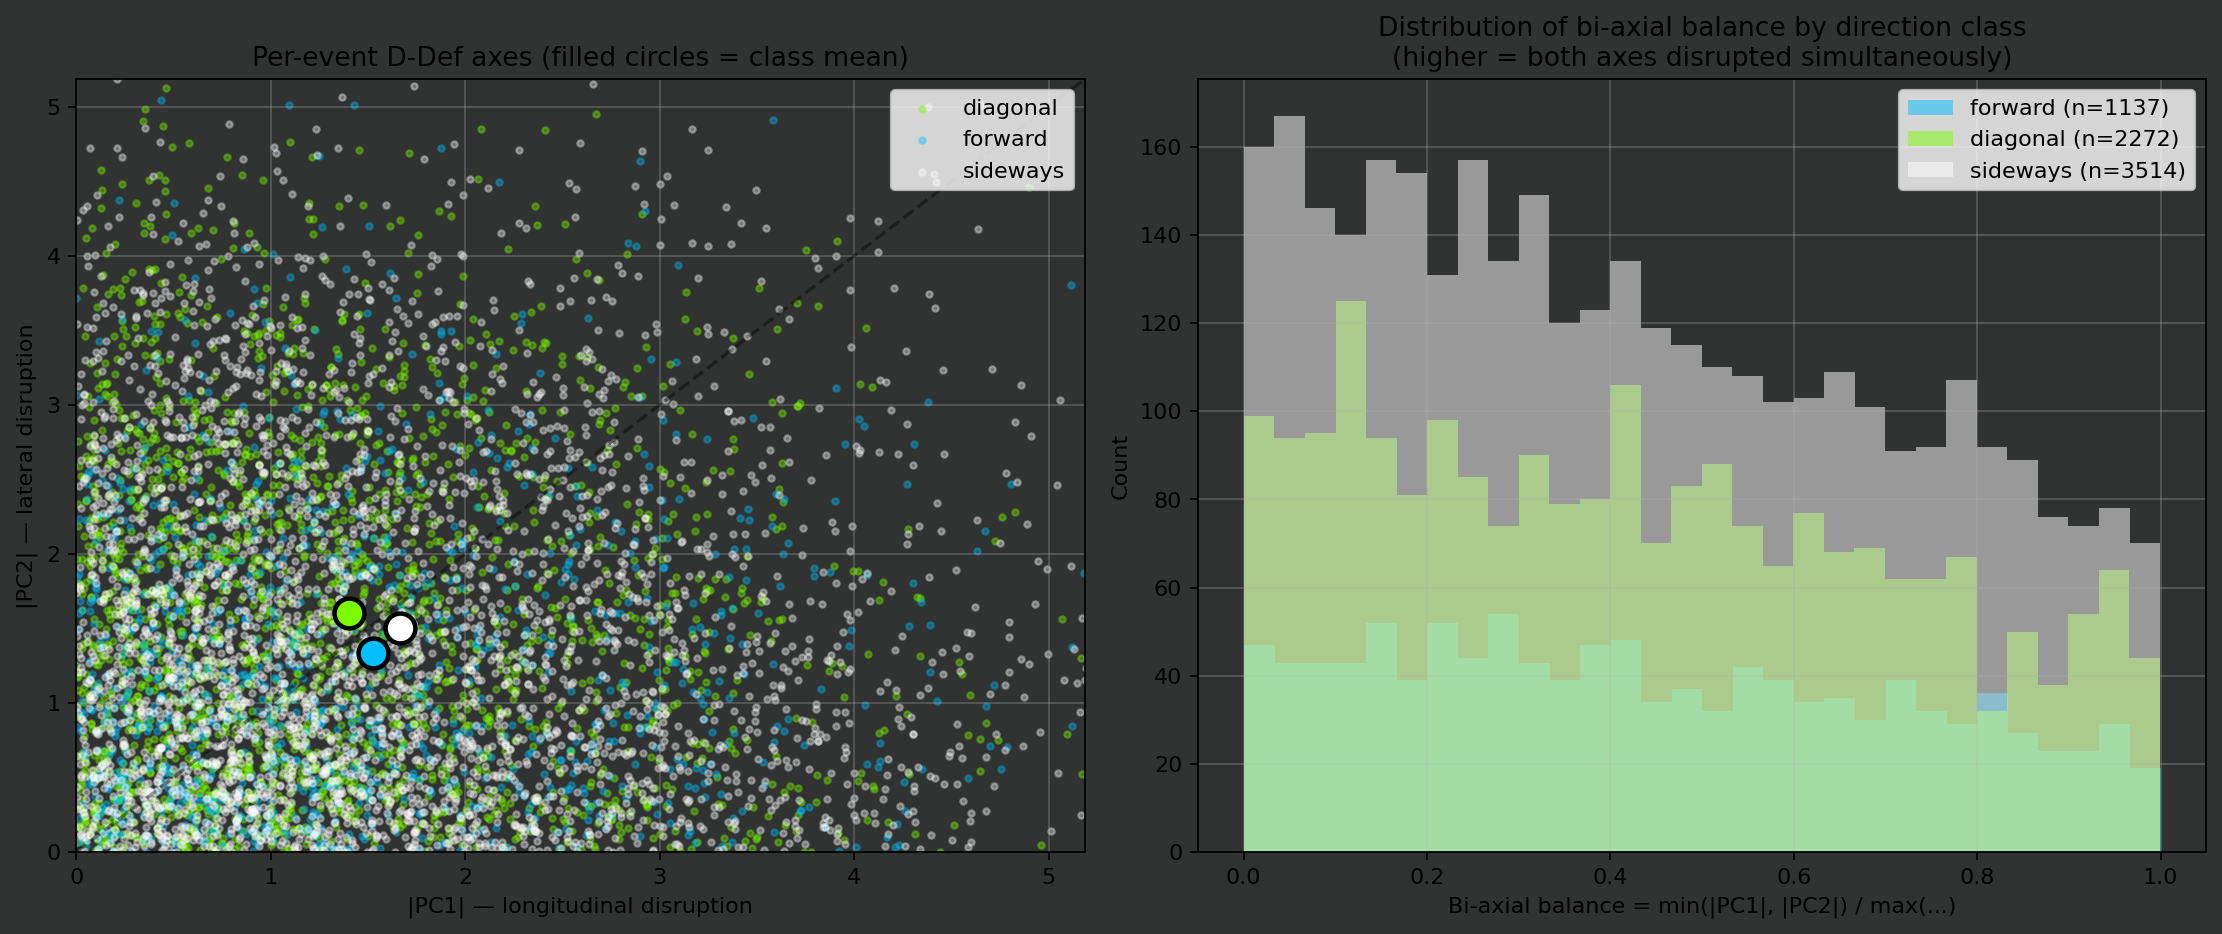
\includegraphics[width=0.97\textwidth]{results_ddef.png}
  \caption{\textbf{Defensive disruption (D-Def, Goes/Forcher).} Per-event
  longitudinal (PC1) vs lateral (PC2) disruption. Diagonal actions are the
  lateral-disruption specialists and carry the highest \emph{combined}
  PC1$+$PC2 disruption.}
  \label{fig:ddef}
\end{figure}

\subsection{Mechanism II --- The Receiver}
\label{sec:res-receiver}

%% PLAN: lado ataque (Aleph del manifiesto + seccion receptor de SV). El
%% receptor de un pase diagonal recibe con el cuerpo casi orientado a
%% porteria: turn-to-goal 108 deg vs 144 deg del forward (p=1.6e-59,
%% rbc=-0.555) y ve mas companeros en su FOV (6.0 vs 5.0, p=6.7e-11). La
%% ventaja diagonal es de PERCEPCION y multiplicidad de opciones.
\begin{figure}[t]
  \centering
  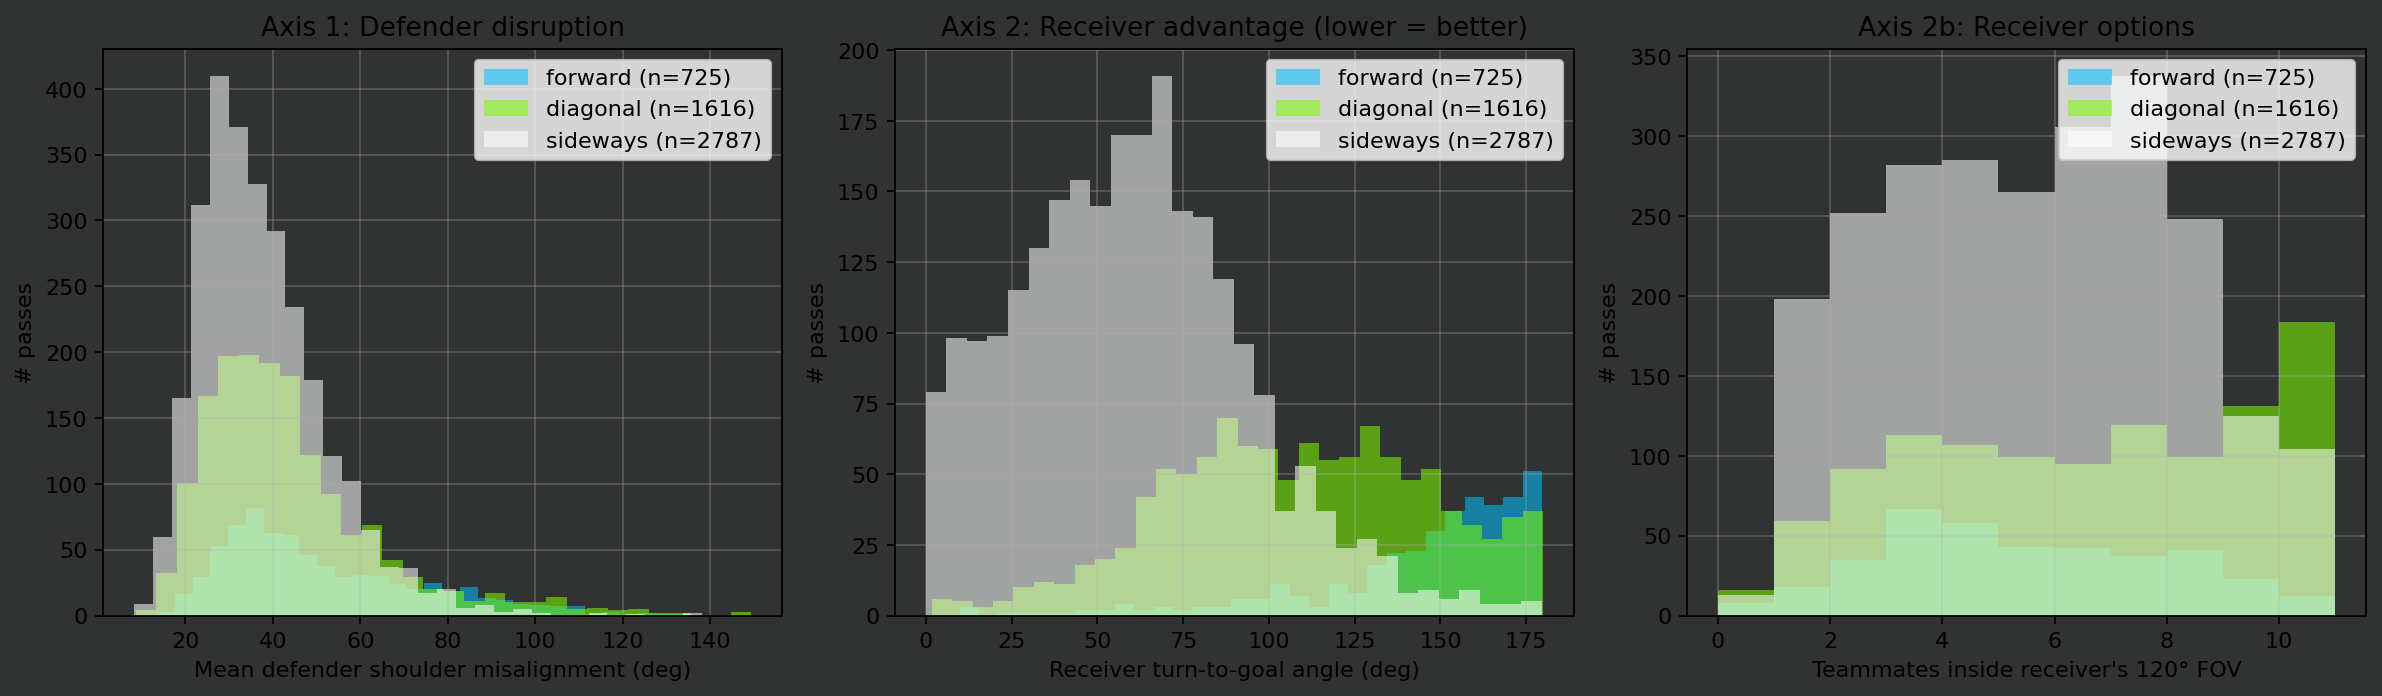
\includegraphics[width=0.97\textwidth]{results_theta.png}
  \caption{\textbf{Receiver advantage.} The receiver of a diagonal pass
  needs far less rotation to face goal and has more team-mates inside the
  120$^\circ$ binocular cone at reception --- Hamilton's point of maximum
  tactical multiplicity.}
  \label{fig:theta}
\end{figure}

\subsection{Case Studies}
\label{sec:res-cases}

%% PLAN: (1) Gol de Kane (Bayern-Hamburg, frame 3585218): recorrer
%% vision -> PPCF -> DOS sobre la misma jugada (Figs 1-3). (2) Mapa de pases
%% de Olise (Fig olise): 62 pases, 82% precision, 24% diagonales.

\begin{figure}[t]
  \centering
  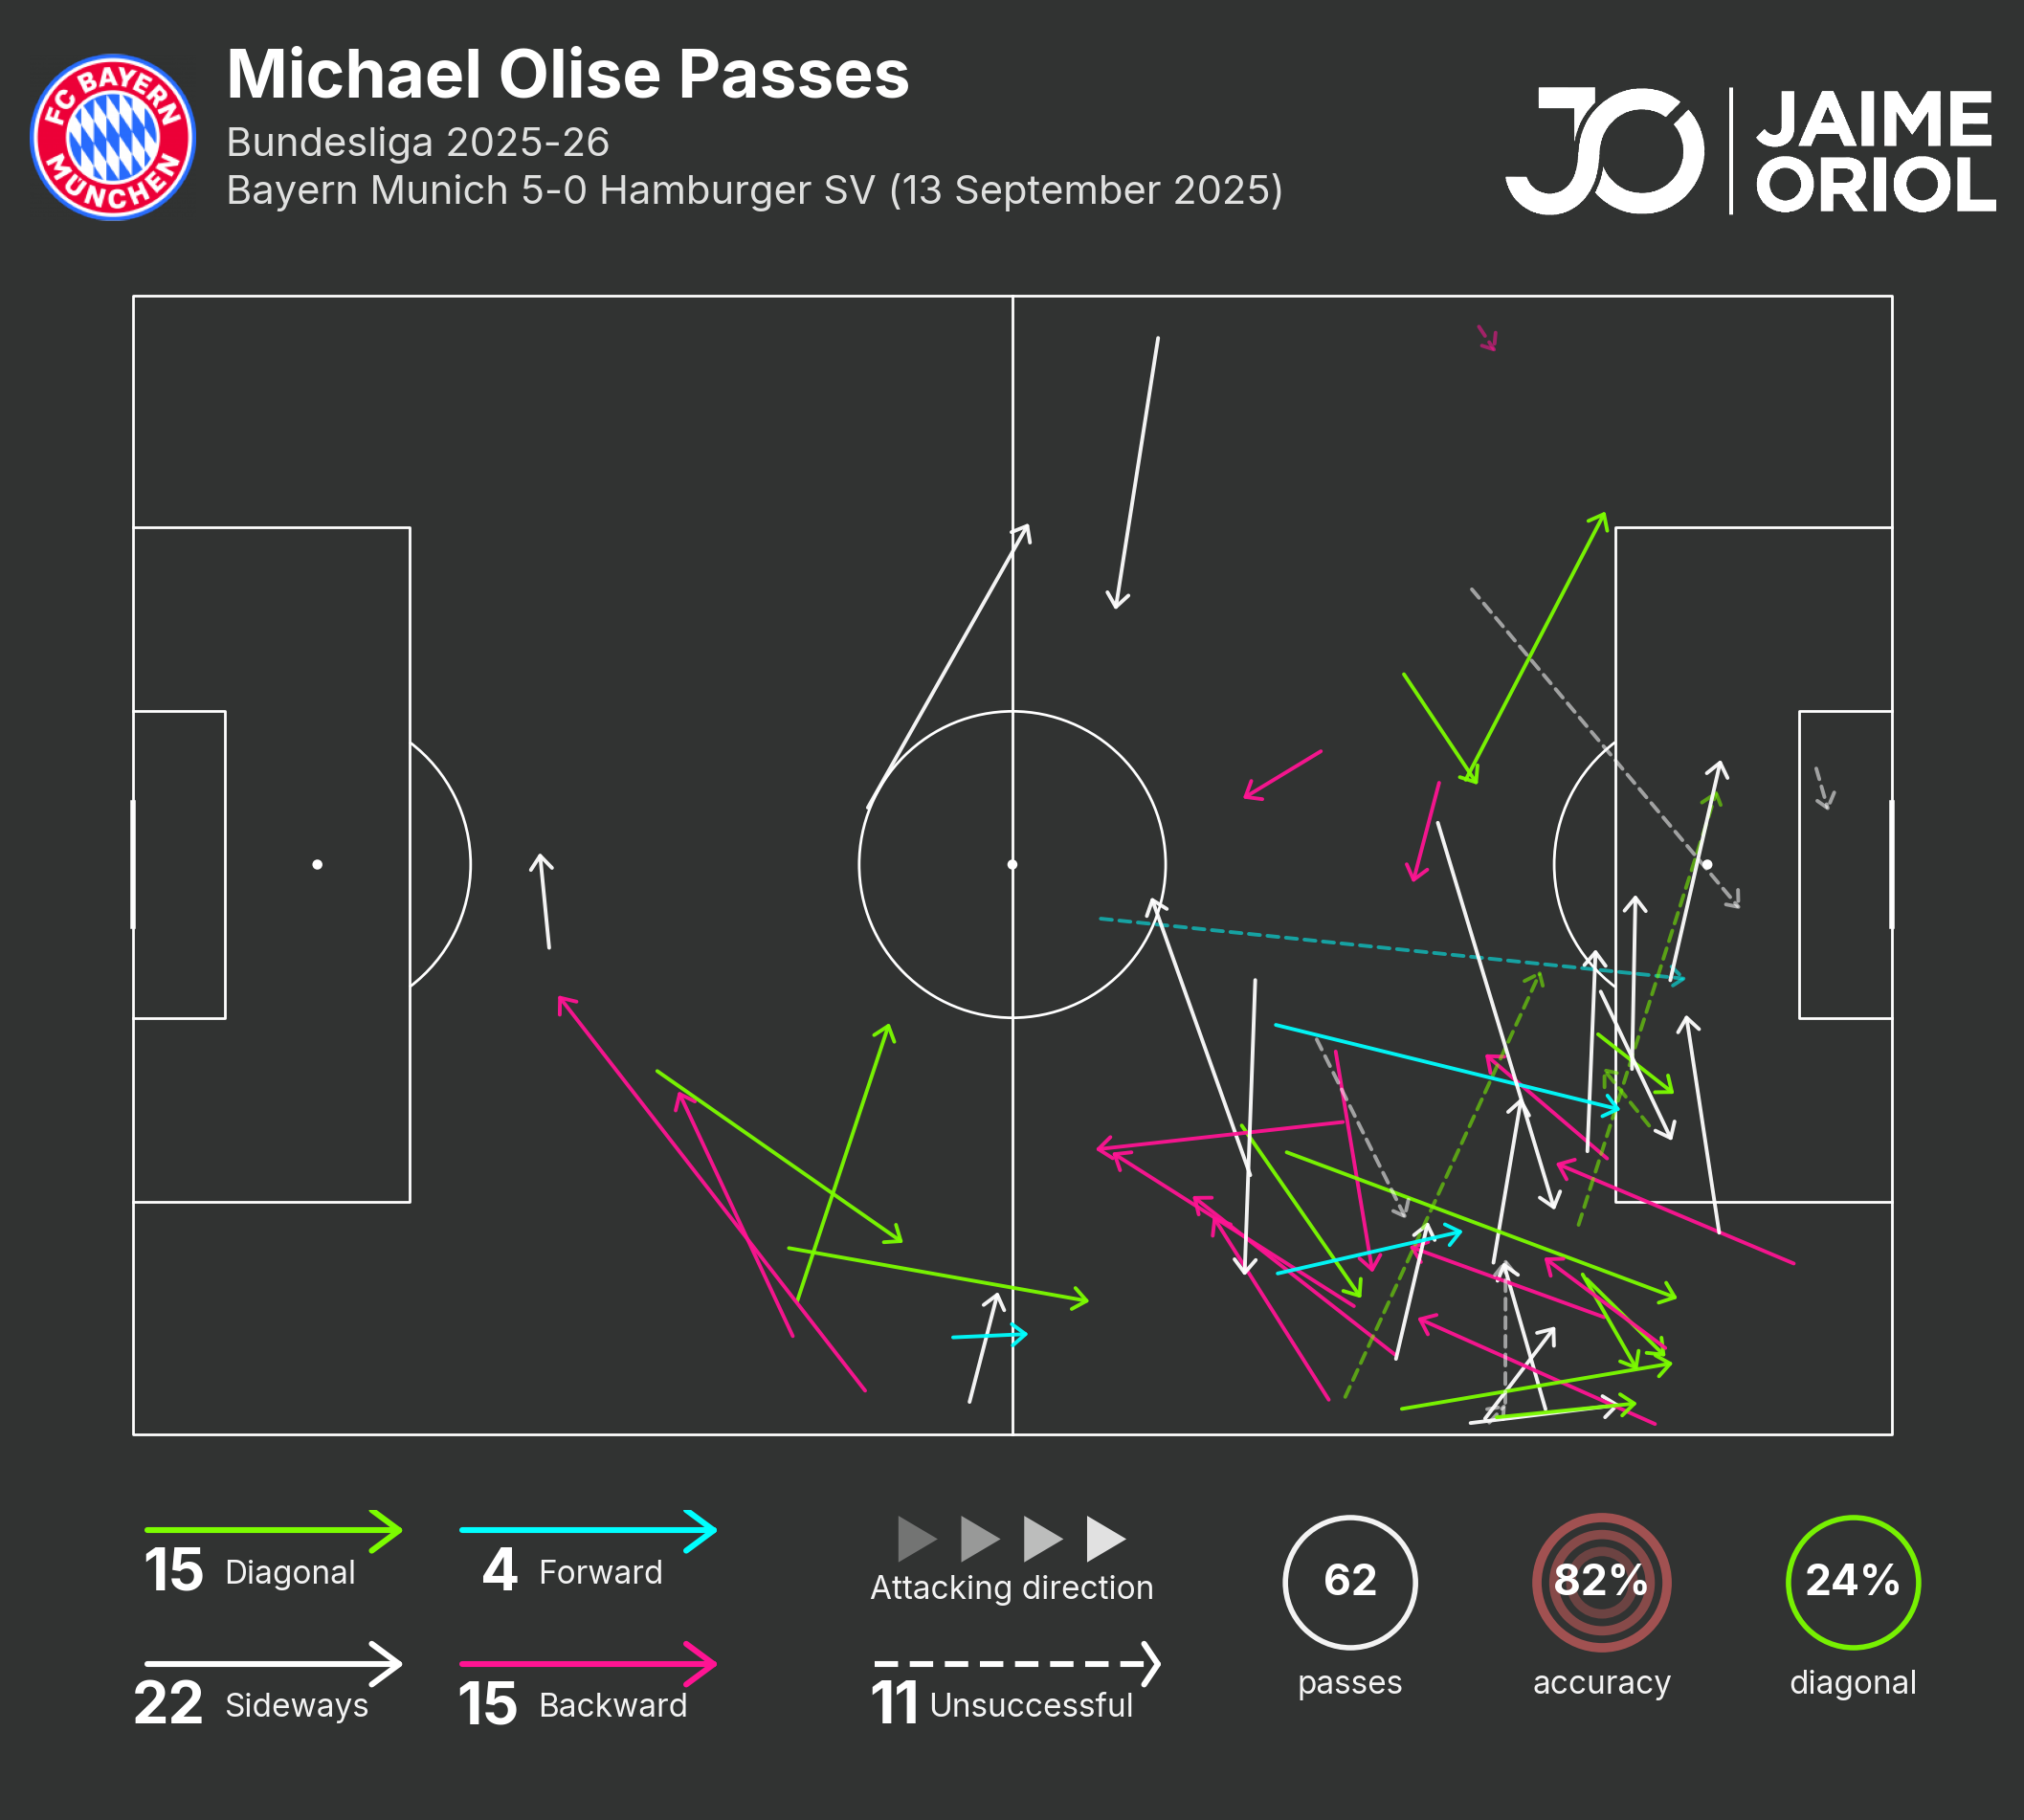
\includegraphics[width=0.78\textwidth]{olise_passes.png}
  \caption{\textbf{Player application: Michael Olise, Bayern 5--0 Hamburg.}
  Pass map coloured by DFL direction class. 62 passes, 82\% accuracy, 24\%
  diagonal. Per-player and per-opponent diagonal profiles are a direct
  scouting output of the framework.}
  \label{fig:olise}
\end{figure}

% =====================================================================
\section{Applications}
\label{sec:applications}

%% PLAN: (i) preparacion de partido - DOS agregada por rival = mapa de
%% vulnerabilidades de orientacion; (ii) post-match - cada accion anotada
%% con theta/DOS; (iii) scouting de jugadores (perfil diagonal, Fig Olise);
%% (iv) broadcast - overlays de vision/blind spot.

% =====================================================================
\section{Limitations and Future Work}
\label{sec:limitations}

%% PLAN honesto: (1) 5 partidos - muestra modesta; (2) OFF-BALL RUNS: el
%% framework vision->PPCF->DOS es agnostico al tipo de accion; lo que falta
%% es el front-end de deteccion de carreras desde la aceleracion del
%% skeleton continuo - es el "nightmare scenario" de Spielverlagerung y el
%% siguiente paso natural; (3) OA-PPCF aun no validada por AUC vs PPCF
%% estandar; (4) la correlacion DOS<->D-Def es negativa: DOS (input de
%% asimetria visual) y D-Def (output estructural) son complementarios, no
%% redundantes - merece estudio.

% =====================================================================
\section{Conclusion}
\label{sec:conclusion}

%% PLAN: la diagonalidad, primera cuantificacion. No es el extremo de ningun
%% eje: es el optimo del trade-off progresion-seguridad. DOS lo convierte en
%% un mapa accionable. "Horizontal keeps you safe; vertical gets you killed
%% or crowned; diagonal lets you decide while still in motion."

% =====================================================================
\bibliographystyle{plainnat}
\bibliography{references}

\end{document}
